\documentclass[a4paper, 12pt]{article}

% input and style
\usepackage[utf8]{inputenc}
\usepackage[T1]{fontenc}
\usepackage[USenglish]{babel}

\usepackage{csquotes}
\usepackage{float}
\usepackage{booktabs}
\usepackage{caption}
\usepackage{graphicx}

\usepackage{hyperref}
\usepackage{url}

% references
\usepackage[
    style=numeric,
    backend=biber,
    natbib=true
]{biblatex}
\addbibresource{main.bib}
\setlength\bibitemsep{10pt}

% math stuff
\usepackage[centertags, sumlimits, intlimits, namelimits]{amsmath}
\usepackage{amssymb}

\DeclareMathOperator*{\SumInt}{%
\mathchoice%
  {\ooalign{$\displaystyle\sum$\cr\hidewidth$\displaystyle\int$\hidewidth\cr}}
  {\ooalign{\raisebox{.14\height}{\scalebox{.7}{$\textstyle\sum$}}\cr\hidewidth$\textstyle\int$\hidewidth\cr}}
  {\ooalign{\raisebox{.2\height}{\scalebox{.6}{$\scriptstyle\sum$}}\cr$\scriptstyle\int$\cr}}
  {\ooalign{\raisebox{.2\height}{\scalebox{.6}{$\scriptstyle\sum$}}\cr$\scriptstyle\int$\cr}}
}

\newcommand{\unitmat}{1\!\!1}

% theorems
\usepackage{amsthm}
\usepackage{xcolor}
\usepackage{mdframed}

\newmdtheoremenv[
    outerlinewidth=2,
    leftmargin=30,
    rightmargin=30,
    innertopmargin=0,
    innerbottommargin=10,
    backgroundcolor=gray!30,
    linecolor=gray,
    nobreak=true
]{conclusion}{Conclusion}[section]

\newtheorem{theorem}{Theorem}
\newtheorem{definition}{Definition}

% title page
\title{default article}
\author{Marcel Köpke}
\date{\today}


\begin{document}

\maketitle

\tableofcontents


\section{Introduction}
\label{sec:introduction}
Sample text: \citep{Bell:1964}



\clearpage
\section{Tables}
\label{sec:tables}
Cite last section \ref{sec:introduction}.

\begin{table}[h]
    \caption{Some caption}
    \centering
    \begin{tabular}{lrrc}
        \toprule
        First row \\
        \midrule
        Column 1 & Column 2 & Column 3 & Column 4\\
        \midrule
        Description & 1 & 2 & 3 \\
        Description & 4 & 55 & 1337 \\
        Description & 7 & 8 & 9 \\
        \bottomrule
    \end{tabular}
    \label{tab:mytable}
\end{table}

More text and reference to table \ref{tab:mytable}.


\clearpage
\section{Equations}
\label{sec:equations}
Some text with this $\sigma = 3$ inline equation.

Some more text with a
$$ \sigma = 3 $$
display equation.

Even more text with a numbered
\begin{equation}
    \sigma = 3
\end{equation}
display equation.

Some text with a
\begin{align}
    \sigma = 3\\
    500 \cdot \sigma =  1500
\end{align}
multiline equation.

Some text with an
\begin{align}
    \sigma & = 3\\
    500 \cdot \sigma & =  1500
\end{align}
aligned equation.

Some text with an aligned equation
\begin{equation}
\begin{aligned}
    \sigma & = 3\\
    500 \cdot \sigma & =  1500
\end{aligned}
\end{equation}
with a single centered number.


\clearpage
\section{Pictures}
\label{sec:pictures}
\begin{figure}[h]
\centering

\includegraphics[scale=0.1]{pic/01.png}
\caption{Small picture}
\end{figure}

\begin{figure}[h]
\centering

\includegraphics[scale=0.5]{pic/02.jpg}
\caption{Normal picture}
\end{figure}

\begin{figure}[h]
\centering
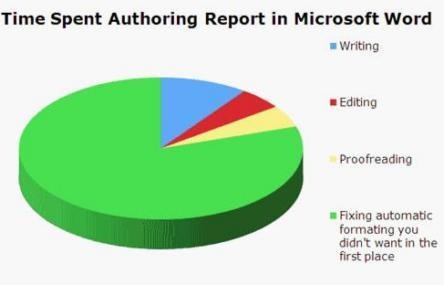
\includegraphics[width=\textwidth]{pic/03.jpg}
\caption{Fit to width}
\end{figure}

\begin{figure}[h]
\centering

\includegraphics[width=6cm, height=0.9\textheight]{pic/04.jpg}
\caption{Stretched}
\end{figure}



\clearpage
\printbibliography

\end{document}

